\documentclass{article}
\usepackage[utf8]{inputenc}
\usepackage{amsmath}
\usepackage{graphicx}
\usepackage{hyperref}
\usepackage[english]{babel}\usepackage{subcaption}
\usepackage{sidecap}
\usepackage{lipsum}
\usepackage{multicol}
\usepackage{sectsty}
\usepackage{caption}
\usepackage{placeins}
\usepackage{subcaption}
\usepackage[dvipsnames]{xcolor}

\definecolor{myred}{RGB}{143, 42, 12}
\definecolor{myblue}{RGB}{58, 83, 197}
\definecolor{myorange}{RGB}{219, 146, 0}
\newcommand{\centered}[1]{\begin{tabular}{l} #1 \end{tabular}}



% \sectionfont{\centering}
\usepackage[a4paper,top=2cm,bottom=2cm,left=2cm,right=2cm]{geometry}
\title{\textbf{Robotics II} \\ \large{\textbf{Final Project}}}
\author{Marco Pennese 1749223}
\date{}

\begin{document}
\maketitle
\tableofcontents
\pagebreak
\section{Denavit-Hartenberg}
\paragraph{}
\FloatBarrier
\begin{table}[!htbp]
\centering
\begin{tabular}{|c|cccc|}
\hline
& $\alpha$ & a & d & $\theta$\\
\hline
link 1 & $\pi$/2 & 0 & $L_1=0.3$ & $q_1$\\
link 2 & 0 & $L_2=0.3$ & $d_2=-0.09$ & $q_2$\\
link 3 & 0 & $L_3=0.2$ & 0 & $q_3$\\
\hline
\end{tabular}
\end{table}
\paragraph{Frame 1}
\begin{center}
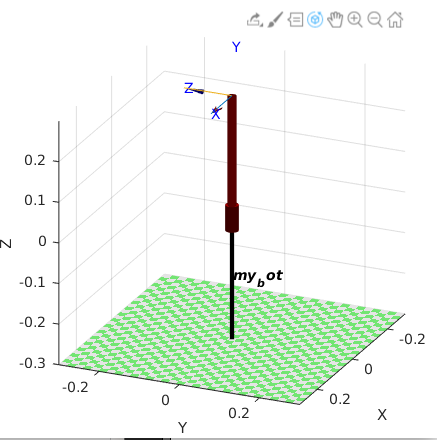
\includegraphics[width=0.5\textwidth]{images/frame1.png}
\end{center}
\paragraph{Frame 2}
\begin{center}
\begin{figure}[!htb]
   \begin{minipage}{0.33\textwidth}
     \centering
     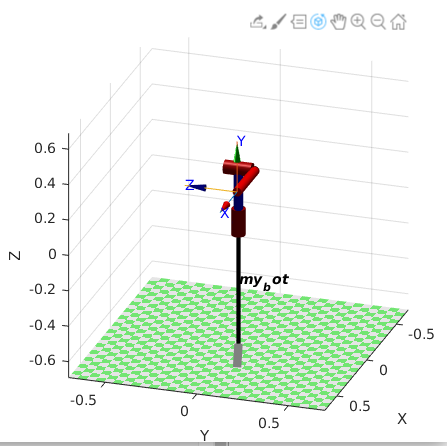
\includegraphics[width=\linewidth]{images/frame2.png}
   \end{minipage}\hfill
   \begin{minipage}{0.33\textwidth}
     \centering
     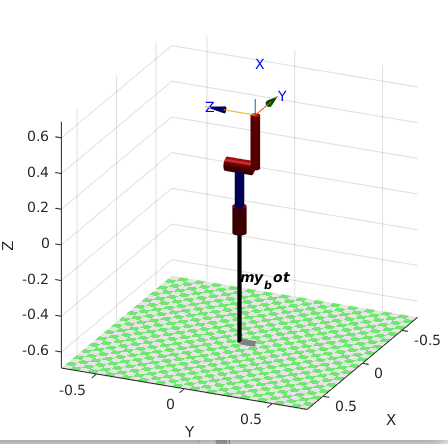
\includegraphics[width=\linewidth]{images/frame2_q2_90.png}
   \end{minipage}\hfill
   \begin{minipage}{0.33\textwidth}
     \centering
     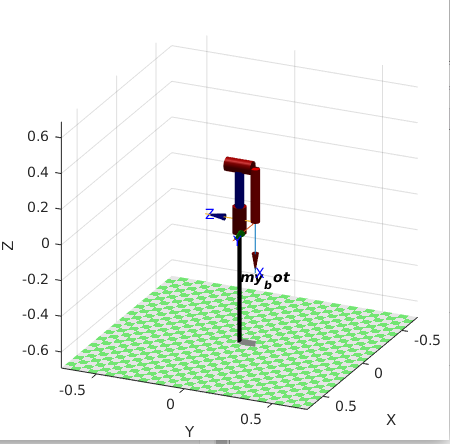
\includegraphics[width=\linewidth]{images/frame2_q2_-90.png}
   \end{minipage}
   \caption{(a) $q_2$ = 0; (b) $q_2$ = 90 deg; (c) $q_2$ = -90 deg}
\end{figure} 
\end{center}
\paragraph{Frame 3}
\begin{center}
\begin{figure}[!htb]
   \begin{minipage}{0.33\textwidth}
     \centering
     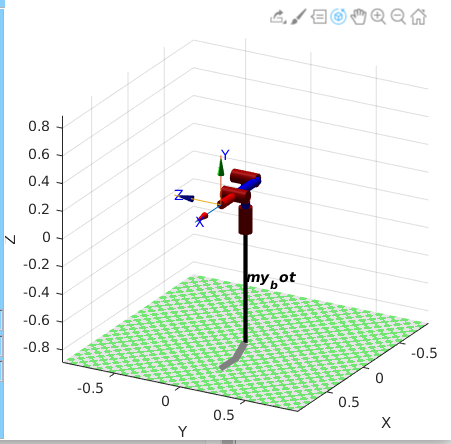
\includegraphics[width=\linewidth]{images/frame3.png}
   \end{minipage}\hfill
   \begin{minipage}{0.33\textwidth}
     \centering
     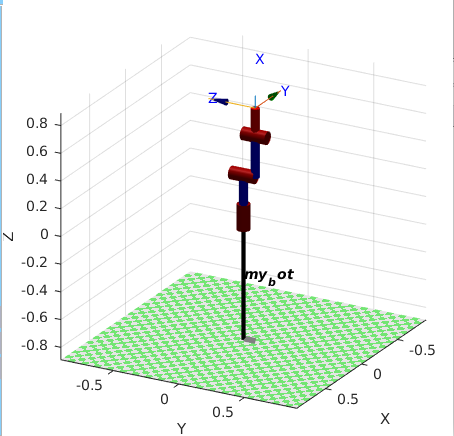
\includegraphics[width=\linewidth]{images/frame3_q2_90.png}
   \end{minipage}\hfill
   \begin{minipage}{0.33\textwidth}
     \centering
     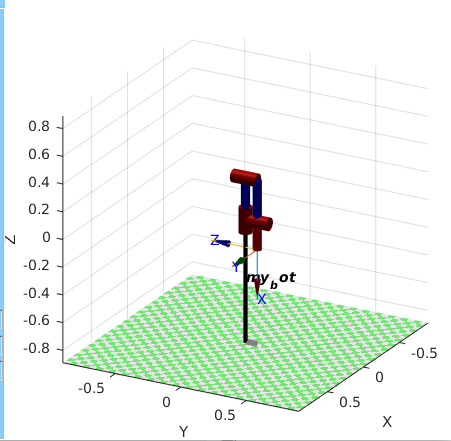
\includegraphics[width=\linewidth]{images/frame3_q2_-90.png}
   \end{minipage}
   \caption{(a) $q_2$ = 0, $q_3$ = 0; (b) $q_2$ = 90 deg, $q_3$ = 0; (c) $q_2$ = -90 deg, $q_3$ = 0}

\end{figure} 
\end{center}
\begin{center}
\begin{figure}[!htb]
   \begin{minipage}{0.33\textwidth}
     \centering
     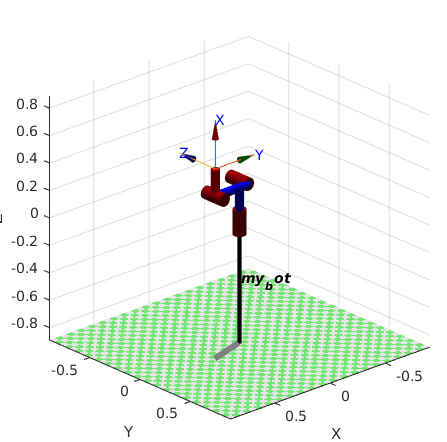
\includegraphics[width=\linewidth]{images/frame3_q2_0_q3_90.png}
   \end{minipage}\hfill
   \begin{minipage}{0.33\textwidth}
     \centering
     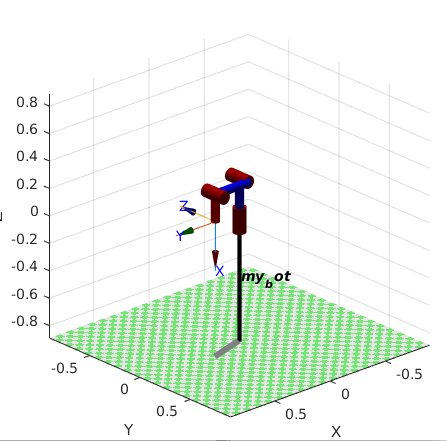
\includegraphics[width=\linewidth]{images/frame3_q2_0_q3_-90.png}
   \end{minipage}\hfill
   \begin{minipage}{0.33\textwidth}
     \centering
     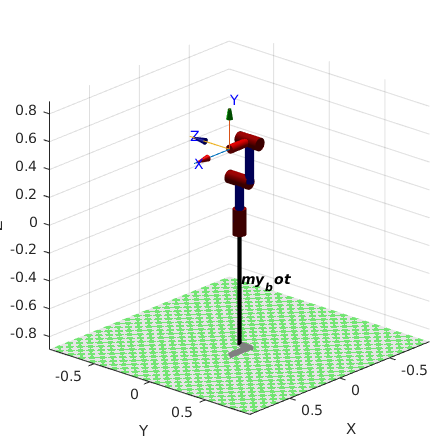
\includegraphics[width=\linewidth]{images/frame3_q2_90_q3_-90.png}
   \end{minipage}
   \caption{(a) $q_2$ = 0, $q_3$ = 90 deg; (b) $q_2$ = 0 deg, $q_3$ = -90 deg; (c) $q_2$ = 90 deg, $q_3$ = -90 deg}

\end{figure} 
\end{center}
\FloatBarrier

\section{Centers of Mass}
asdfg
\end{document}
